\documentclass{article}

\usepackage{graphicx}
\usepackage{tikz}
\usepackage{tikzsymbols}
\usetikzlibrary{calc,patterns,shapes.geometric}
\pagestyle{empty}
\usepackage[margin=0pt]{geometry}
\geometry{papersize={14in,12in}}

\def\centerarc[#1](#2)(#3:#4:#5){\draw[#1] ($(#2)+({#5*cos(#3)},{#5*sin(#3)})$) arc (#3:#4:#5);}

\begin{document}
	\begin{figure}
		\centering
		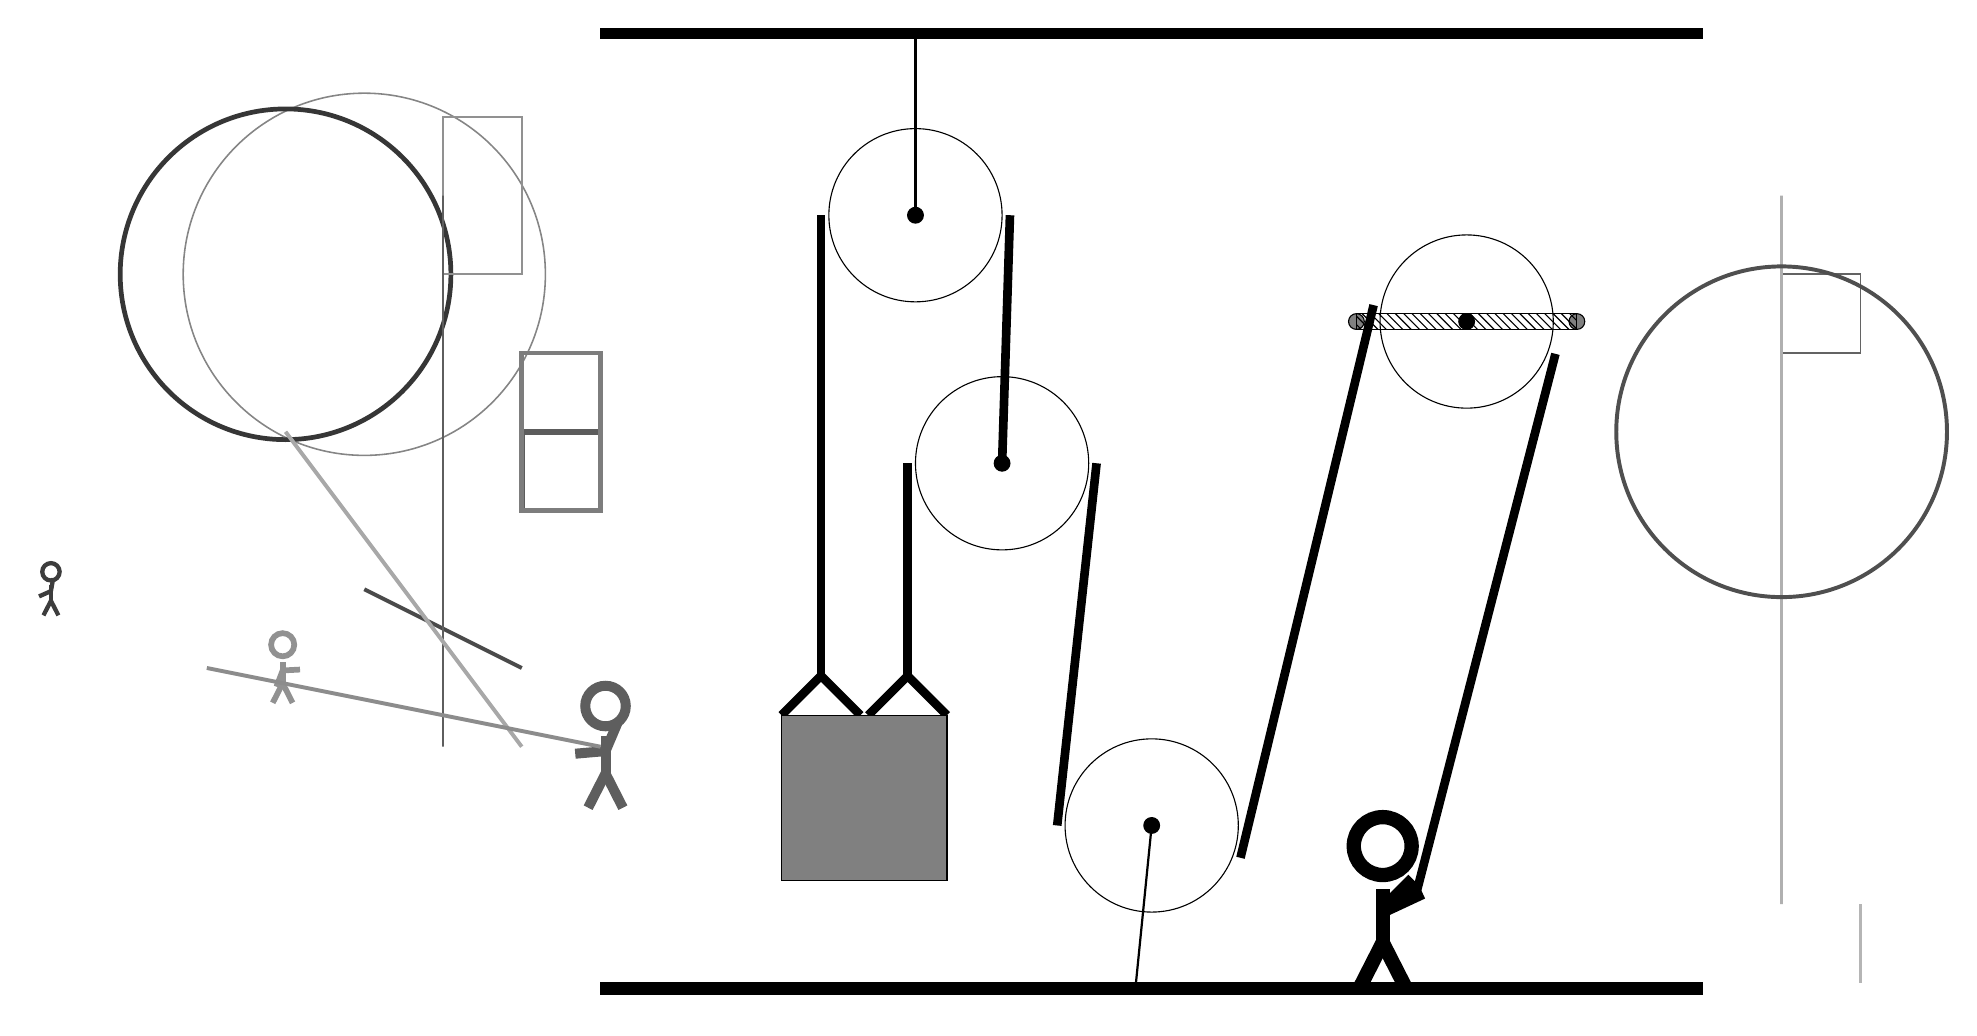
\begin{tikzpicture}
			%%%%% START %%%%%
			
			\draw[fill=black] (-2, 9) rectangle (12, 9.125);
			
			\draw (2, 6.75) circle (1.1);
			\draw[fill=black] (2, 6.75) circle (0.1);
			\draw[thick] (2, 6.75) -- (2, 9);
			
			\draw (3.1, 3.6) circle (1.1);
			\draw[fill=black] (3.1, 3.6) circle (0.1);
			
			\draw (5, -1) circle (1.1);
			\draw[fill=black] (5, -1) circle (0.1);
			\draw[thick] (5, -1) -- (4.8, -3);
			
			\draw (9, 5.4) circle (1.1);
			\draw[fill=black] (9, 5.4) circle (0.1);
			\draw[fill=black!50] (7.6, 5.4) circle (0.1);
			\draw[fill=black!50] (10.4, 5.4) circle (0.1);
			\draw[pattern=north west lines, pattern color=black] (7.6, 5.5) rectangle (10.4, 5.3);
			
			\draw[line width = 1.1mm]  (0.3, 0.4) -- (0.8, 0.9) -- (1.3, 0.4);
			\draw[line width = 1.1mm]  (1.4, 0.4) -- (1.9, 0.9) -- (2.4, 0.4);
			\draw[fill=black!50] (0.3, 0.4) rectangle (2.4, -1.7);
			
			\draw[line width = 1.1mm] (0.8, 6.75) -- (0.8, 0.9);
			\centerarc[line width = 1.1mm](2, 6.75)(0:180:1.2000000000000002);
			\draw[line width = 1.1mm] (3.2, 6.75) -- (3.1, 3.6);
			\draw[line width = 1.1mm] (1.9, 3.6) -- (1.9, 0.9);
			\centerarc[line width = 1.1mm](3.1, 3.6)(0:180:1.2000000000000002);
			\draw[line width = 1.1mm] (4.3, 3.6) -- (3.8, -1);
			\centerarc[line width = 1.1mm](5, -1)(180:340:1.2000000000000002);
			\draw[line width=1.1mm](6.1276, -1.4104) -- (7.8182, 5.6083);
			\centerarc[line width = 1.1mm](9, 5.4)(-20:170:1.2000000000000002);
			\draw[line width=1.1mm](10.1276, 4.9896) --  (8.35, -1.9);
			
			\draw[line width=0.2mm, color=black!61] (13, 5) rectangle (14, 6);
			
			\node[line width=0.2mm, color=black!63] at (-2, 0) {\Strichmaxerl[7][5][67]};
			\draw [line width=0.2mm, color=black!48](-5, 6) circle (2.3);
			\draw[line width=0.7mm, color=black!64] (-2, 3) rectangle (-3, 4);
			\draw [line width=0.6mm, color=black!79](-6, 6) circle (2.1);
			\draw[line width=0.5mm, color=black!71](-5, 2) -- (-3, 1);
			
			\draw[line width=0.2mm, color=black!43] (-4, 8) rectangle (-3, 6);
			
			\draw[line width=0.4mm, color=black!29] (14, -2) rectangle (14, -3);
			\node[line width=0.2mm, color=black!76] at (-9, 2) {\Strichmaxerl[3][24][80]};
			\draw[line width=0.6mm, color=black!51] (-2, 3) rectangle (-3, 5);
			\draw[line width=0.3mm, color=black!63] (-4, 0) rectangle (-4, 7);
			\draw[line width=0.5mm, color=black!34](-3, 0) -- (-6, 4);
			\node[line width=0.3mm, color=black!43] at (-6, 1) {\Strichmaxerl[4][69][3]};
			\draw[line width=0.5mm, color=black!45](-2, 0) -- (-7, 1);
			\draw[line width=0.3mm, color=black!31] (13, -2) rectangle (13, 7);
			\draw [line width=0.5mm, color=black!69](13, 4) circle (2.1);
			
			\node at (8, -2) {\Strichmaxerl[10][225][25]};
			
			\draw[fill=black] (-2, -3) rectangle (12, -3.15);
			
			%%%%% END %%%%%
		\end{tikzpicture}
	\end{figure}	
\end{document}